\documentclass[12pt]{article}
\usepackage[czech]{babel}
\usepackage[utf8]{inputenc}
\usepackage[IL2]{fontenc}
\usepackage{wrapfig}
\usepackage{graphicx}
\usepackage{cprotect}
\usepackage{amsmath}


\begin{document}
%\setlength{\parindent}{0pt}
\begin{titlepage}

\includegraphics[scale=0.2, trim=5cm 0 0 30cm]{logo.jpg}
\begin{center}
\vspace{5cm}
{\Huge
\textbf{KIV/ZVI}\\
\vspace{1cm}
}
{\Large
\textbf{PŘÍZNAKOVÉ ROZPOZNÁVÁNÍ OBJEKTŮ VE SNÍMKU}
}
\end{center}
\vspace{\fill}

\begin{minipage}[t]{5cm}
\flushleft
Martin Hamet\\
\end{minipage}
\hfill
\begin{minipage}[t]{7cm}
\flushright
\today
\end{minipage}
\end{titlepage}

\tableofcontents
\newpage
\section{Zadání}
\label{zadani}
Nad zadanými obrazovými daty ve formátu BMP, 512 x 512 obrazových bodů, 256 úrovní šedé,
v souborech IMG.BMP proveďte úlohy:

\begin{itemize}
\renewcommand\labelitemi{--}
\setlength\itemsep{1px}
\item Zvolenou metodou segmentace obrazu nalezněte všechny objekty ve snímku, určete jejich počet
a jednotlivé objekty označte (např. obarvením plochy).
\item Určete vnitřní hranice jednotlivých objektů, vypočítejte obvod a těžiště pro každý objekt.
\item Metodami příznakového rozpoznávání nalezněte zadané objekty ( písmena a číslice zadané z klávesnice ), příznakový vektor může obsahovat např.: polohu těžiště, obvod, plochu opsaného
čtyřúhelníka, počet děr, členitost hraniční čáry, ...
\item Testování bude prováděno na natočených objektech a po provedení opakované dilatace, resp. eroze (do úrovně, kdy ještě nebude narušena topologie objektů) a po rozostření obrazu průměrováním v okolí 5 x 5.
\item Procedury pro dilataci, erozi a průměrování snímku budou součástí programové realizace.
\end{itemize}


\section{Analýza problému a návrh řešení}
Úkolem je demonstrace jednotlivých metod a jejich použití pro klasifikaci objektů ve snímku. Úlohu lze rozdělit tři hlavní části segmentaci, parametrizaci a klasifikaci. Segmentací získámé jednotlivé prvky obrazu. Pomocí parametrizace zajistíme jednotný popis individuálních objektů, který bude možné dále klasifikovat
pomocí klasifikátoru. 

Protože se jedná o demonstrační úlohu, bylo by vhodné konstruovat ji s vědomím že by se mohla v budoucnu rozšiřovat o další metody (klasifikátory, způsoby segmentace etc.).

\pagebreak
\subsection{Segmentace}
\label{segmentation}
Segmentace se zabývá identifikací objektů ve snímků obvykle na základě nějaké vlastnosti, která je objektu vlastní. Objektem se v našem případě myslí znak (tvar) v obrazu, který se vyznačuje vysokou hodnotou jasu vůči svému okolí. Tedy světlé objekty na tmavém pozadí. Jednotlivé pixely můžeme tedy označit za součást objektu pokud jejich hodnota jasu překročí jistou hranici.

Pro učení prahové hodnoty lze použít automatické algoritmy, nicméně vzhledem k povaze našich vstupních dat, kde jsou obrázky stejného formátu s podobným jasovým rozložením, prahovou hodnotu určíme experimentálně a nebude ji třeba nadále upravovat.

K vlastnímu oddělení objektů od pozadí lze použít různě metody např. spojováním oblastí, maticí sousednosti, etc. V našem případě se jednotlivé objekty nekříží, ani nejsou vnořené (objekt obsahující jiný objekt). Nejsme tolik omezeni komplexností snímku a můžeme použít méně obvyklý způsob založený na Freemanově řetězovém kódu (viz \ref{Freeman_use}). Tento způsob nám zajistí nalezení celého objektu podle jeho vnitřní hranice. 

\subsubsection{Freemanův řetězový kód a jeho využití pro segmentaci}
\label{Freeman_use}

\paragraph{Freemanův řetězový kód}
Jedná se obecně o způsob popisu spojité křivky respektive posloupnosti jejích jednotlivý bodů. Lze uvažovat o sousednosti typu \texttt{D} (4 - okolí) nebo \texttt{DI} (8 - okolí). Protože nemáme žádné zvláštní požadavky na popis hranice použijeme \texttt{D} okolí pro hledání sousedních bodů. 

\begin{wrapfigure}[12]{r}{9cm}
\centering
\vspace{-0.5cm}
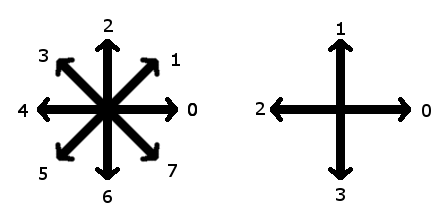
\includegraphics[height=4cm]{Freeman_dir.png}
\caption{Popis směru ve Freemanově řetězovém kódu \texttt{DI}(vlevo) \texttt{D}(vpravo).}
\label{freeman_dir}
\end{wrapfigure}

Popis je založen na popisu směru ve kterém se nachází další sousední bod. Z praktického pohledu není třeba uchovávat informace o každém bodu hranice, ale pouze o počátku a dále jen informaci o směru k dalšímu bodu. Použitím omezeného počtu směrů (\texttt{D} okolí) se zabýváme pouze čtyřmi směry, které můžeme zakódovat jednocifernou číslicí (viz obr.\ref{freeman_dir}).

\paragraph{Využití pro segmentaci}
Pro nalezení objektu využijeme Freemanova kódu tak, že budeme procházet jednotlivé body obrazu a při nalezení bodu, který lze považovat za součást objektu (viz. \ref{segmentation}), přejdeme na problém popisu vnitřní hranice objektu.

\begin{wrapfigure}[16]{l}{7cm}
\centering
\vspace{-0.0cm}
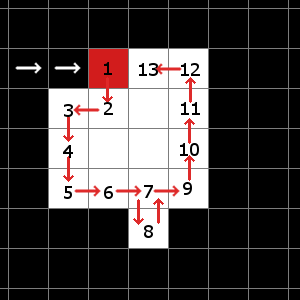
\includegraphics[height=6cm]{Freeman_edge.png}
\caption{Pohyb po vnitřní hranici objektu.}
\label{freeman_edge}
\end{wrapfigure}

Chceme-li popisovat vnitřní hranici musíme stanovit pravidla pro hledání následujícího bodu tak, aby tento bod byl také bodem hranice. Pokud tedy budeme procházet obrázkem zleva doprava a shora dolu tak nevyhnutelně prvním nalezeným bodem bude levý horní roh objektu \texttt{1}(viz obr. \ref{freeman_edge}). Budeme postupovat proti hodinovému směru. V průběhu průchodu si budeme držet informaci v jakém směru jsme našli aktuální bod. Pro \texttt{1} si určíme směr dolů (směr č. 3 viz obr. \ref{freeman_dir}). Nový bod budeme hledat vždy v pořadí očíslování směrů a začneme o jeden směr zpět od směru ze kterého jsme nalezli aktuální bod. Například bod \texttt{3} jsme nalezli ve směru doleva (\texttt{2}) tedy kontrolujeme sousedy v pořadí (horní (\texttt{1}), levý (\texttt{2}), dolní (\texttt{3}) a pravý (\texttt{4})) a označíme dolního souseda jako další hraniční bod \texttt{4} nalezený ve směru dolů (\texttt{3}). Tímto způsobem máme zajištěný průchod všech hraničních bodů nalezeného objektu a tím i definováním jeho umístění ve snímku. 

\subsubsection{Označení zpracovaných bodů}
Při výše popsaném průchodu snímkem by docházelo k opakovanému průchodu jíž nalezených objektů, proto je nutné všechny body, které byli označeny jako součásti objektů (včetně vnitřních) označit jako již zpracované.

Pro nalezení vnitřních bodů daného objektu můžeme využít samotného průchodu po hranici a ukládat indexy nalezených hraničních bodů. Protože předpokládáme že nedochází ke křížení objektů, ani k jejich vnořování můžeme si dovolit ukládat pouze minimální a maximální index (Například pro třetí řádek v obr. \ref{freeman_edge} by jsme si uložili index prvku \texttt{3} při jeho průchodu a index prvku \texttt{11}. 

Takto získáme popis objektu podobný \texttt{RLC} s tím rozdílem že máme pouze počáteční a koncový index pro jednotlivé řádky. Všechny body mezi těmito indexy, které lze považovat za součást objektu, patří tomuto objektu a můžeme je tedy označit za nalezené.

\subsection{Parametrizace}
\label{Parametrization}
Parametrizace slouží jako jednotný popis vybraných vlastností objektu, který se dá dále použít pro klasifikaci. Pro snadné uložení a zpracování těchto vlastností bude vhodné použít tzv. parametrizační vektor kde jeho složky jsou hodnoty odpovídající jednotlivým vlastnostem daného objektu.

Efektivita (popisová síla) jednotlivých vlastností se těžko určuje a je silně závislá na povaze objektů, které chceme popisovat. Protože objekty mohou mít náhodnou rotaci nemá smysl volit spojené s pozicí ve snímku, což značně sníží popisovací a tím i rozlišovací schopnost aplikace.

\subsubsection{Minimální opsaný čtyřúhelník}
\label{minRectangle}
\begin{wrapfigure}[9]{r}{7.3cm}
\centering
\vspace{-0.25cm}
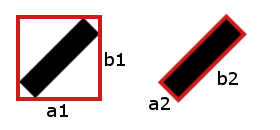
\includegraphics[height=3cm]{MinRectangle.png}
\caption{Minimální opsaný obdélník.}
\label{minRectangle_obr}
\end{wrapfigure}
Parametry opsaného obdélníku získáme snadno, pokud si uložíme minimální a maximální souřadnice respektive jejich složky \texttt{X, Y} jednotlivých bodů hranice. Body obdélníku budou:\\ \texttt{[min X, min Y]}, \texttt{[min X, max Y]}, \texttt{[max X, max Y]}, \texttt{[min X, max Y]}.

Chceme-li minimální opsaný obdélník musíme vzít v úvahu úhel otočení objektu (viz obr. \ref{minRectangle_obr}). Všechny údaje potřebné pro takový čtyřúhelník lze získat například rotací bodů na hranici se zvoleným krokem (nejlépe násobením transformační maticí) a hledání minimálních a maximálních souřadnic jak bylo popsáno dříve. Porovnáním obsahů takto získaných obdélníků získáme přibližně minimální s přesností podle zvoleného kroku.

Protože minimální opsaný čtyřúhelník není závislý na rotaci je to vhodný výchozí bod pro množství dalších parametrů objektu.

\subsubsection{Podlouhlost}
Z minimálního opsaného čtyřúhelníka (viz \ref{minRectangle}) můžeme snadno získat tzv. podlouhlost , která udává poměr jeho delší a kratší strany \texttt{b2/a2} dle obr. \ref{minRectangle_obr}.

\subsubsection{Obsah}
\label{volume}
Obsah objektu lze spočítat pomocí všech bodů, které danému objektu patří, respektive jejich jasů. Lze využít vážený obsah, kdy budeme brát v úvahu úroveň jasu v každém pixelu, nebo pouze pixelů patřících objektu. Protože jsou jasy vstupních dat víceméně uniformní budeme uvažovat druhou možnost. Aby jsme snížili závislost na velikosti objektu bude vhodnější získaný obsah vydělit obsahem minimálního obdélníku (viz \ref{minRectangle}). Získáme tím více univerzální popis než samotným obsahem.

\subsubsection{Težiště}
Těžiště lze počítat vážené, nebo brát všechny body patřící objektu se stejnou vahou podobně jako obsah (viz \ref{volume}). Pokud vezmeme nevážené těžiště jedná se o průměrné souřadnice všech bodů patřících objektu. Aby jsme snížili závislost na pozici a rotaci objektu vztáhneme souřadnice těžiště vůči minimálnímu opsanému čtyřúhelníku. Toho docílíme rotací těžiště v úhlu rotace obdélníku (rotujeme podle stejného bodu jako při hledání obdélníku např. střed bitmapy) a odečtením hodnot souřadnic např. levého horního rohu. 

Dále protože je možné najít minimální čtyřúhelník ve čtyřech možných úhlech rotace bude vhodné vztáhnout souřadnice těžiště ještě k rozměrům obdélníku ve smyslu kratší a delší strany v daném pořadí. Výsledné dvě hodnoty tedy získáme z rotovaného bodu těžiště:
\begin{equation} \label{eq1}
d_1 = \frac{x - xr}{Min\{w, h\}} \qquad
d_2 = \frac{y - yr}{Max\{w, h\}}
\end{equation}
Kde [$x$, $y$] jsou souřadnice rotovaného těžiště, [$xr$, $yr$] jsou souřadnice levého horního rohu minimálního obdélníku, $w$ a $h$ jsou jeho šířka a výška.

\pagebreak
\subsubsection{Nejdelší spojnice}
\label{longLine}
Jedná se o nejdelší rozměr mezi dvěma body hranice v objektu. Tento údaj lze získat porovnáním všech dvojic bodů na hranici. Aby tento údaj nebyl přímo závislý na velikosti objektu vztáhneme ho ke kratší (delší) straně minimálního obdélníku vydělením touto hodnotou.

\subsubsection{Kruhovitost}
Udává jakousi podobnost zkoumaného objektu a kruhu. Form factor spočítáme podle následujícího vztahu:

\begin{equation} \label{eq2}
F = 4\pi\frac{S}{O^2}
\end{equation}

Kde $S$ je obsah objektu a $O$ jeho obvod. Obvod získáme jednoduše, protože máme hranici objektu spojitou ve smyslu \texttt{D} okolí obvod je tedy počet prvků hranice.

\subsubsection{Počet děr}
Jako díru uvažujeme spojitou oblast, ve smyslu \texttt{D} okolí, která je plně obklopena objektem. Jinými slovy nedotýká se hranice snímku.
K nalezení takových oblastí lze využít více způsobů. Protože zpracováváme relativně malé obrázky (objekty) můžeme využít rekurentního přístupu. Jeho hlavní výhodou je jednoduchost. Nevýhoda vzniká při zpracování většího snímku může nastat problém s nedostatečnou velikostí zásobníku.

Hledání spočívá v rekurzivním průchodu všemi pixely snímku, kde každý nově objevený pixel označíme jako nalezený (nebude se znovu zpracovávat) a pokud narazíme na pixel na hranici snímku zavrhneme celou nalezenou oblast, která tedy není dírou. Dále vybereme další nenalezený pixel a pokračujeme v průchodu. Pokud se tedy rekurentním pohybem ve smyslu \texttt{D} okolí z počátečního bodu nedá dostat na hranici snímku jedná se o díru.

Počet děr objektu je závislý pouze na spojité topologii objektu a je tedy ideálním parametrem pro popis. Nemá bohužel žádnou popisovací (rozlišovací) schopnost mezi znaky (objekty) bez děr.

\subsection{Klasifikace}
Při parametrizaci jsme získali vektor pro každý objekt, který ho podle zvolených parametrizačních metod popisuje. V klasifikační části potřebujeme určit do jaké klasifikační třídy zařadit vektor na základě trénovacích dat, kde jsme znali správný výsledek. Je tedy třeba klasifikátor připravit (vytvořit model) v trénovací části tak, aby s co největší přesností určil správnou třídu bez znalosti výsledku. Klasifikátor musí být také schopen takto vytvořený model uložit a případně později načíst, proto budeme volit jednoduché datové struktury. Pro účely ukládání bude vhodnější formát XML místo TXT vzhledem k přehlednosti uložených dat.

\subsubsection{Etalonový klasifikátor}
Tento klasifikátor nejprve načte všechna trénovací data a poté je zpracuje a vytvoří vzorové parametrizační vektory pro každou klasifikační třídu. Při testování už pouze počítá vzdálenost vzorů (etalonů) od testovaného vektoru (ze zkoumaného objektu). Podle etalonu s nejkratší vzdáleností od testovaného zařadí testovaný vektor do příslušné třídy. Jedná se o jednoduchý klasifikátor, kde ovšem záleží na správném vytvoření etalonů.

Nejjednodušší způsob určení etalonů je průměr v dané klasifikační třídě z vektorů vytvořených z trénovacích dat. Výhodou je že po trénovací fázi není nutné uchovávat všechna trénovací data, ale pouze výše zmíněné etalony a je tedy tento klasifikátor paměťově výrazně úsporný.

Pro vypočítání vzdálenosti v našem případě příznakových vektorů můžeme použít Euklidovskou vzdálenost. Je důležité aby se po celou dobu funkce tohoto klasifikátoru používal stejný parametrizační algoritmus, který produkuje vektory o stejné délce což je zajištěno parametrizací (viz \ref{Parametrization}).

\pagebreak
\section{Implementace (popis řešení)}
V této sekci budou popsány hlavní moduly programu a jejich vzájemná funkce. Třídy a procedury nutné pro vykreslování a práci s GUI nebudou popisovány vzhledem k jejich nevýznamnosti vůči řešenému problému. Nicméně jsou nezanedbatelnou součástí aplikace.
\\(třídy \texttt{Form1} hlavní okno a \texttt{FragmentDetailForm} okno detailu objektu)

\subsection{\texttt{Program}}
Zajišťuje hlavní řízení programu.
\paragraph{\texttt{main()}}
Vstupní bod programu vytvoří příslušné prvky konzole, GUI a předá řízení hlavnímu oknu \texttt{Form1}.
\paragraph{\texttt{evaluateBitmap()}}
Vyhodnotí bitmapu, všechny objekty které obsahuje a vyplní jejich příslušné popisy. Výsledky jsou zobrazeny v hlavním okně aplikace.

\subsection{Image}
Jedná se o obalovou třídu, která shromažďuje veškeré informace o snímku a poskytuje funkce pro práci sním a objekty které daný snímek obsahuje.

\paragraph{\texttt{process()}}
Hlavní metoda volaná z konstruktoru zajistí průchod bitmapy snímku a nalezení objektů které obsahuje použitím metody \texttt{processByFreeman()}. Základní informace o jednotlivých objektech jsou uloženy do jejich instancí \texttt{Image.Fragment}.

\paragraph{\texttt{openBitmap()}}
Zajišťuje umožnění přístupu přímo k datům bitmapy. Je nutné po skončení práce volat metodu pro uzavření \texttt{closeBitmap()}.

\subsubsection{Image.Fragment}
Jedná se o obalovou třídu obsahující veškeré informace o nalezeném objektu (body vnitřní hranice, počátek, rozměry, etc.).

\subsection{Description}
Obalová třída pro detailní informace o objektu vyplněné především při generování parametrizačního vektoru. Slouží pro předání informací o objektu do GUI.

\subsection{DefaultDescriptor}
Slouží pro generování parametrizačního vektoru pro daný objekt. 

\paragraph{\texttt{getDescription()}}
Vytvoří parametrizační vektor a nastaví všechny příslušné údaje objektu v obalové třídě \texttt{Description}. Vektor je dále vynásoben váhami jednotlivých parametrů po složkách.

\paragraph{\texttt{setAttributes()}}
Nastaví atributy minimálního opsaného čtyřúhelníka v \texttt{Description}, které budou potřeba pro generování parametrizačního vektoru.

\subsection{DistanceClassifier}
Reprezentuje etalonový klasifikátor. Přidávané trénovací vektory ukládá do seznamů ve slovníkové struktuře tak, že klíčem je správná klasifikační třída. Při prvním zavolání metody \texttt{evaluate()} se projdou všechny trénovací vektory metodou \texttt{compileReadings()} a vytvoří se příslušné etalony do seznamu \texttt{finalPatterns}. Při ukládání modelu zanikají informace o trénovacích vektorech a ukládá se pouze seznam etalonů.

\paragraph{\texttt{addTrainCase()}}
Přidá do klasifikátoru nový vektor se správnou třídou. Pomocí opakovaného volání této metody se trénuje klasifikátor.

\paragraph{\texttt{evaluate()}}
Vytvoří vektor (descriptorem klasifikátoru) z předaného objektu \texttt{Image.Fragment} a klasifikuje ho. Metoda vrací řetězec představující výsledek klasifikace (odpovídající klasifikační třídu).

\paragraph{\texttt{saveModel()}}
Uloží natrénovaný model do souboru (\texttt{Model.data}) ve formátu \texttt{XML} pro pozdější použití.

\section{Uživatelská příručka}
Pro správný běh programu je nutné, aby se spustitelný soubor nacházel ve stejném adresáři jako složka s testovacími daty, případně uložený soubor \texttt{Model.data}. Dále program vyžaduje nainstalovaný \texttt{Microsoft.NET Framework}.

\subsection{Spuštění programu}
Program je samostatně spustitelný a běžná komunikace probíhá pomocí uživatelského rozhraní (viz \ref{GUI}).
Program také lze spustit z příkazové řádky pro některé stavové výpisy, ale není to z běžného pohledu nutné.

\subsubsection{Formát uložených dat}
\paragraph{Vstupní snímek}
Očekávaný velikost vstupních obrázků je \texttt{512x512} pixelů. Není nezbytně nutné tento parametr dodržet, ale s většími obrázky značně roste riziko spadnutí programu kvůli použití rekurzivního řešení a tedy vysokých nároků na paměť. Formát pixelů vstupního snímku by měl být \texttt{8bppIndexed} (8bitů na pixel s indexací).

\paragraph{Trénovací data}
Musí být uložena tak, že složka \texttt{TrainingData} obsahuje podsložky s názvy správných klasifikačních tříd, aby bylo jasné co za třídu klasifikátor právě trénuje (tyto názvy budou použity jako výsledky klasifikace). V těchto složkách se nacházejí jednotlivé snímky příslušící dané třídě.

\paragraph{Datový model}
Model je uložený ve formátu \texttt{XML} jako soubor \texttt{Model.data}. V souboru jsou uložené informace o použitém klasifikátoru a descriptoru. Dále následuje datový blok \texttt{<patterns>}, kde jsou uloženy jednotlivé ethalony parametrizačních vektorů pro každou klasifikační třídu. Parametrizační vektor je složen s hodnot které odpovídají parametrům vektoru  pořadí: \{obsah, podlouhlost, těžiště-1, těžiště-2, sppojnice-1, spojnice-2, kruhovitost, počet děr\}. Jednotlivé hodnoty jsou vynásobeny složkami váhového vektoru \{1, 2, 2, 2, 0.5, 0.5, 2.5, 3.5\}.


\pagebreak
\subsubsection{Grafické uživatelské rozhraní GUI}
\label{GUI}

\paragraph{Hlavní okno}
Po spuštění GUI je okamžitě možné sním pracovat. Nejprve je nutné natrénovat klasifikátor pomocí tlačítka \texttt{Train Classifier}, nebo načíst již hotový ze souboru \texttt{Load Classifier}.

Po vytvoření (načtení) klasifikátoru se zpřístupní možnost otevření vstupního snímku \texttt{Open Image}. Otevřený snímek bude zobrazen v hlavním panelu. S otevřeným snímkem je možné pracovat pomocí tlačítek:
\begin{itemize}
\renewcommand\labelitemi{--}
\setlength\itemsep{1px}
\item{\texttt{Blur 5x5}} Rozmazání průměrováním pomocí masky o rozměrech \texttt{5x5}.
\item{\texttt{Dilatation}} Dilatace obrázku maskou \texttt{D} okolí.
\item{\texttt{Erosion}} Eroze obrázku maskou \texttt{D} okolí.
\item{\texttt{Step back}} Zajišťuje funkci návratu o jeden krok zpět.
\item{\texttt{Evaluate}} Vyhodnotí obrázek a zobrazí v nalezené objekty jako výslednou klasifikační třídu a souřadnice levého horního rohu opsaného čtyřúhelníka.
\item{\texttt{Detail}} Otevře nové okno s detailem vybraného objektu ze seznamu.
\end{itemize}

\paragraph{Okno detailu}
Okno je určené pro zobrazení detailů jednoho objektu ze snímku. Těchto oken je možné mít otevřeno více. V okně se nachází výpis některých důležitých parametrů objektu a pomocí tlačítek lze některé zobrazit přímo v objektu.

\begin{itemize}
\renewcommand\labelitemi{--}
\setlength\itemsep{1px}
\item{\texttt{Show Original}} Zobrazí originální výřez z původního snímku.
\item{\texttt{Show Minimal Rectangle}} Vykreslí minimální opsaný čtyřúhelník oranžovou barvou.
\item{\texttt{Show Edge}} Zvýrazní červeně vnitřní hranici objektu.
\item{\texttt{Show Center of Gravity}} Oranžovým křížem naznačí těžiště objektu.
\end{itemize}


\section{Testování}
Testování jednotlivých parametrizačních metod a algoritmu segmentace není dokumentovaná vzhledem k jednoduchému ověření pomocí přiložených obrázků ve složce \texttt{TestIndividual} a zobrazením detailu v uživatelském rozhraní (viz \ref{GUI}).

\subsection{Testování klasifikátoru}
Testování klasifikace bylo provedeno na zadaných datech s využitím metod pro dilataci a rozmazání. Ve snímku se nachází 15 objektů úspěšnost klasifikace je tedy vztažená k tomuto počtu. Natočený snímek byl vždy klasifikován po použití funkce rozmazání.
\vspace{0.5cm}


\begin{tabular}{|c|c|}
$\texttt{Úroveň dilatce}$ & $\texttt{Úspěšnost}$\\\hline
$1$ 	& $89\%$ 		\\\hline
$2$ 	& $83\%$		\\\hline
$3$ 	& $66\%$		\\\hline
$4$ 	& $63\%$		\\\hline
$5$ 	& $63\%$		\\\hline
$6$ 	& $56\%$		\\\hline
\end{tabular}
\begin{tabular}{|c|c|}
$\texttt{Úroveň eroze}$ & $\texttt{Úspěšnost}$\\\hline
$1$ 	& $93\%$ 		\\\hline
$2$ 	& $86\%$		\\\hline
$3$ 	& $73\%$		\\\hline
$4$ 	& $56\%$		\\\hline
$5$ 	& $49\%$		\\\hline
$6$ 	& $49\%$		\\\hline
\end{tabular}

\section{Závěr}
Program je připraven pro další rozšiřování o klasifikátory a parametrizační algoritmy. Zvolené algoritmy byly vybrány tak, aby byly snadno implementovatelné a dali se dále rozšiřovat. Vzhledem k tomu že vstupní formát pixelů (\texttt{8bppIndexed} není standardně podporován základními funkcemi, bylo nutné pracovat na mnohem nižší úrovni abstrakce, přestože pracujeme s relativně malými snímky. 

Jednotlivé parametrizační metody byli snadno ověřitelné pomocí uměle vytvořených snímků (o několika pixelech).
Samotná klasifikace není příliš efektivní především kvůli jednoduchosti zvoleného klasifikátoru, absenci rozsáhlých trénovacích dat a pokročilejších trénovacích algoritmů. Přesto se podařilo dosáhnout alespoň částečné klasifikační schopnosti aplikace. Kvůli rotaci vstupních snímků nebylo možné využít vyzkoušené metody (např. histogram orientovaných gradientů), které silně závisí na pozici a jejich zobecněné verze se neprojevili jako příliš efektivní (alespoň v jejich jednoduché verzi).

Testování klasifikace bylo provedeno na zadaných datech s využitím metod pro dilataci a rozmazání.
\end{document}